\section{Realizarea lucrarii de laborator}

\subsection{Tasks and Points}
\begin{itemize}
	\item Basic Level (nota 5 || 6):
	
	\begin{itemize}
		\item Realizeaza un simplu GUI calculator care suporta functiile de baza: +, -, /, *.
	\end{itemize}
	
	\item Normal Level (nota 7 || 8):
	
	\begin{itemize}
		\item Realizeaza un simplu GUI calculator care suporta urmatoare functii: +, -, /, *, putere, radical, InversareSemn(+/-).
	\end{itemize}
	\item Advanced Level (nota 9 || 10):
	
	\begin{itemize}
		\item Realizeaza un simplu GUI calculator care suporta urmatoare functii: +, -, /, *, putere, radical, InversareSemn(+/-), operatii cu numere zecimale.
	\end{itemize}
	\begin{itemize}
		\item Divizare proiectului in doua module - Interfata grafica(Modul GUI) si Modulul de baza(Core Module).
	\end{itemize}
\end{itemize}
\subsection{Analiza lucrarii de laborator}

Linkul la repozitorul Github:\\
\begin{center}
\url{https://github.com/dmitrii724/MIDPS}
\end{center}

Am realizat Calculatorul folosind IDE-ul Visual Studio 2015 Community in limbajul \textsc{\large C\#} folosind un proiect de tip Windows Forms Application.Calculatorul final:\\
\begin{center}
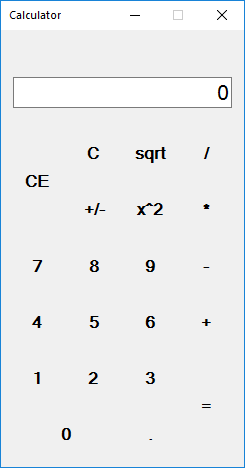
\includegraphics[scale=1]{images/1}
\end{center}
Pentru a realiza interfata grafica a calculatorului am utlizat paleta de componente din Visual Studio si le-am amplasat in fereastra generata initial la crearea proiectului.La calculator am utilizat doar trei componente:button,TextBox si Label.Butoanele predestinate pentru operatii,TextBox pentru afisarea rezultatelor si cifrele care sunt introduse utilizind mouse-ul si tastatura, si Label-ul pentru afisarea cifrelor si operatiilor curente.Cind selectam un buton in modul grafic putem modifica(caption,color,font,style,name...) din Diolog-Boxul din dreapta numit Properties.La realizarea functionalul pentru butoane am utilizat functii globale care extrag din cimpul text a butonului valoarea pentru a fi utilizata la calcule.Utilizind functii universale am optimizat codul,in rezultat nu a fost necesar sa implementez functii pentru fiecare button.Am divizat actiunile butoanelor in cinci functii:butoane-Cifre(button\_Click),butoane-Operatii(operator\_Click),butonul-CE(buttno16\_Click),butonul-C(button17\_Click) si butonul-$=$(button18\_Clik).Operatiile 
$+,-,*,/$ sunt chemate la actiunea butonuli egal care prelucreaza operatiile in baza funtiiei universale operator\_Click.

\section{Imagini}
Imaginea finala a calculatorului creat.
\begin{center}
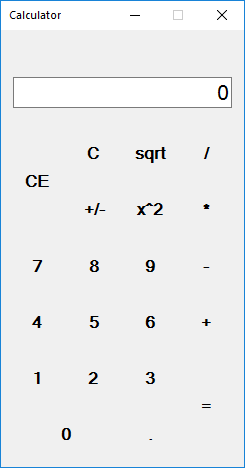
\includegraphics[scale=1]{images/1}
\end{center}
\clearpage